\begin{figure}[!h]
\centering
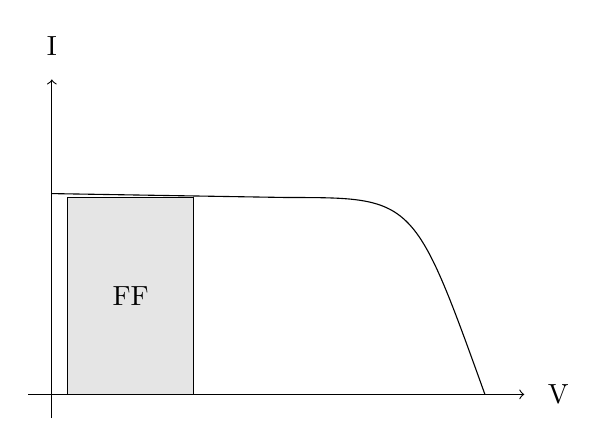
\begin{tikzpicture}

	\draw [->] (-0.3,0) -- (6,0) node [right=5pt]	{V};  % X-akse
	\draw [->] (0,-0.3) -- (0,4) node [above=5pt]	{I}; % Y-akse

	% Faktisk kurve
	\draw [-] (0,2.55) -- (3,2.5);
	\draw [-] (3,2.5) .. controls +(right:1.6cm) .. (5.5,0);
	% Fyllfaktor
	\node [draw, rectangle,fill=black!10,minimum height=2.5cm, minimum width=1.6cm] (FF) at (1,1.25) {FF};
	
\end{tikzpicture}

\caption{Str�m-spenningskarakterisitikken for en solcelle}%
\label{fig:ivsolcelle}%
\end{figure}